\documentclass[12pt]{article}
\usepackage[T1]{fontenc}
\usepackage[utf8]{inputenc}
\usepackage[croatian]{babel}
\usepackage{amsmath}
\usepackage{graphicx}
\usepackage{hyperref}
\usepackage{listings}
\usepackage{listings}
\usepackage{color} % For coloring code (optional)
\usepackage{tikz}
\usetikzlibrary{arrows}
\usetikzlibrary{automata, positioning}

\lstset{
	language=Matlab,
	basicstyle=\ttfamily,
	breaklines=true,
	keywordstyle=\color{blue},
	stringstyle=\color{red},
	commentstyle=\color{green},
	morecomment=[l][\color{magenta}]{\#}
}


\title{Izvještaj: Laboratorijska vježba za skrivene Markovljeve modele}
\author{Dominik Barukčić}
\date{\today}

\begin{document}
	
	\maketitle
	
	% MATLAB Kod
%	\subsubsection*{MATLAB Kod}
%	\begin{lstlisting}
%		
%		a = 10;
%		b = 20;
%		c = a + b;
%		disp(c);
%	\end{lstlisting}
%	
%	% Rezultati
%	\subsubsection*{Rezultati}
%	Ovdje navedite rezultate izvršavanja koda.
%	
%	% IZVJEŠTAJ
%	\subsubsection*{IZVJEŠTAJ}
%	Ovdje odgovorite na pitanja, komentirajte rezultate, i sl. ovisno o tekstu pod-zadatka.
	
	
	U izradi.
	
	\section{Opis eksperimenta}
	Odabrani stohastički eksperiment je temeljen na bacanju tri pristrane igrače kocke s mogućim ishodima bacanja od 1 do 6. Ove kocke su „podešene“ na način da će prva kocka u prosjeku, u pola svih bacanja dati broj „1“, da će druga kocka također u pola svih bacanja dati broj „3“ i da će treća na jednak način u pola svih bacanja dati broj „5“. Vjerojatnosti preostalih ishoda bacanja bitno su manje, ali nisu jednake, nego su ovisne o pojedinoj kocki za svaki od preostalih 5 mogućih brojeva. Ishod bacanja kocke vidljiv je gledateljima, dok ono što im nije vidljivo jest informacija koja od tri pristrane kocke je korištena pri pojedinom bacanju, pa stoga indeks korištene kocke (1., 2. ili 3. kocka) predstavlja skriveno stanje ovog modela.
	
	Promjene skrivenih stanja definirane su prijelaznom matricom modela, pri čemu neki prijelazi u ovom eksperimentu nisu dozvoljeni, tj. imaju nultu vjerojatnost. Konkretno, ako je u aktualnom bacanju korištena prva kocka, tada će u narednom bacanju biti korištena ta ista kocka, ili druga kocka, ali ne može biti odabrana treća kocka. Analogno, ako je model u stanju bacanja druge kocke, može ostati u tom stanju, ili prijeći u stanje treće kocke, ali se ne može vratiti u stanje prve kocke. Konačno kada uđe u stanje treće kocke, može ciklički prijeći u stanje prve kocke, ili ostati u postojećem stanju, ali se ne može vratiti u stanje druge kocke. Zaključno, ovaj model nužno ciklički prolazi kroz skrivena stanja 1->2->3->1, uz mogućnost zadržavanja u aktualnom stanju. Vjerojatnost zadržavanja istog stanja iznosi (M-1)/M, dok vjerojatnost prijelaza u naredno cikličko stanje iznosi 1/M.
	
	\begin{center}
		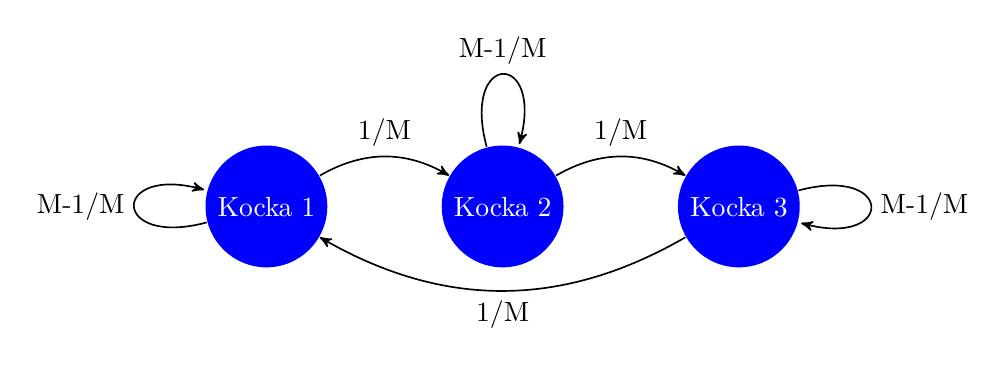
\begin{tikzpicture}[->, >=stealth', auto, semithick, node distance=3cm]
			\tikzstyle{every state}=[fill=blue,draw=none,text=white]
			
			\node[state] (A) {Kocka 1};
			\node[state] (B)[right of=A] {Kocka 2};
			\node[state] (C)[right of=B] {Kocka 3};
			
			\path
			(A) edge[bend left] node[above] {1/M} (B)
			edge[loop left] node {M-1/M} (A)
			(B) edge[bend left] node[above] {1/M} (C)
			edge[loop above] node {M-1/M} (B)
			(C) edge[bend left] node[below] {1/M} (A)
			edge[loop right] node {M-1/M} (C);
		\end{tikzpicture}
	\end{center}
	
	U svrhu definiranja početnog stanja ovog modela, dakle samo za prvo bacanje, koristi se dodatna nepristrana kocka na ovaj način: ako je ishod bacanja te nepristrane kocke „1“ za prvo bacanje će se koristiti prva pristrana kocka, za ishode „2“ ili „3“ koristit će se druga kocka, dok se u slučaju preostala tri ishoda, „4“, „5“ i „6“, kao prva baca treća pristrana kocka.
	
	\section{Opis zadanog modela}
	Slučajni eksperiment kojeg koristimo za ovu vježbu odnosi se na bacanje tri pristrane igrače kocke, gdje indeks korištene kocke predstavlja skriveno stanje ovog HMM modela. Vjerojatnosti pojedinih ishoda bacanja su različite za svaku pristranu kocku, a vjerojatnosti cikličke izmjene stanja su određene parametrom M. Za detaljni opis eksperimenta svakako pogledajte opis vježbe u ranije navedenom dokumentu.
	
	Zadani parametar zadržavanja istog stanja iznosi M=5.
	
	Matrica prijelaznih i početnih vjerojatnosti HMM modela zadane su kao:
	
	\begin{equation}
		A = \begin{bmatrix}
			4/5 & 1/5 & 0 \\
			0 & 4/5 & 1/5 \\
			1/5 & 0 & 4/5
		\end{bmatrix}
	\end{equation}
	
	
	\begin{equation}
		P = \begin{bmatrix}
			1/6 \\
			1/3 \\
			1/2
		\end{bmatrix}
	\end{equation}
	
	
	Prosječne učestalosti osmatranja pojedinih ishoda "1" do "6" za sve tri kocke u 40 bacanja su:
	
	\begin{equation}
		B\_count =\begin{bmatrix}
			20 & 4 & 5 & 2 & 4 & 5 \\
			5  & 4 & 20 & 5 & 3 & 3 \\
			1  & 2 & 5 & 7 & 20 & 5
		\end{bmatrix}
	\end{equation}
	
	
	\section{Pod-zadaci}
	
	\subsection{Pod-zadatak 1: Definiranje HMM Modela}
		% Tekst zadatka
	Temeljem zadanih ucestalosti pojedinih ishoda bacanja pristranih kocki i temeljem zadanog parametra M u vasem Moodle zadatku,
	potrebno je dopuniti predlozak Matlab skripte kako bi cjelovito opisali zadani HMM model ovog eksperimenta ukljucujuci i matricu
	vjerojatnosti osmatranja izlaznih simbola.
	
	% MATLAB Kod
	\subsubsection*{MATLAB Kod}
	\begin{lstlisting}
		
		a = 10;
		b = 20;
		c = a + b;
		disp(c);
	\end{lstlisting}
	
	% Rezultati
	\subsubsection*{Rezultati}
	Ovdje navedite rezultate izvršavanja koda.
	

	
	\subsection{Pod-zadatak 2: Log-Izvjesnosti Osmotrenih Nizova}
	Osmotrena su dva niza duljine T=41 simbola kojeg je generirao model L:\newline
	O = [o1 .. oT] = \newline
	[ 3 6 6 4 5 1 2 3 5 4 4 5 5 3 1 6 1 5 3 5 5 5 4 5 5 5 6 5 1 6 1 3 3 3 3 3 6 3 4 1 3]\newline 
	[ 2 2 3 5 3 6 3 4 4 4 4 1 4 6 1 4 2 6 4 1 4 3 2 5 6 6 6 4 6 6 2 6 6 3 4 4 4 2 3 4 2]\newline
	(2a) Izračunajte log-izvjesnosti osmatranja ova dva niza uz zadane parametre HMM modela te ih upišite u naredna dva polja:
	
	\subsubsection*{MATLAB Kod}
	\begin{lstlisting}
		
		a = 10;
		b = 20;
		c = a + b;
		disp(c);
	\end{lstlisting}
	
	% Rezultati
	\subsubsection*{Rezultati}
	Ovdje navedite rezultate izvršavanja koda.\newline
	\newline
	(2b) Izračunajte i upišite u Moodle koliko puta je drugi niz manje izvjestan od prvog u eksponencijalnom zapisu:
	
	% MATLAB Kod
	\subsubsection*{MATLAB Kod}
	\begin{lstlisting}
		
		a = 10;
		b = 20;
		c = a + b;
		disp(c);
	\end{lstlisting}
	
	% Rezultati
	\subsubsection*{Rezultati}
	Ovdje navedite rezultate izvršavanja koda.
	
	% IZVJEŠTAJ
	\subsubsection*{IZVJEŠTAJ}
	Možete li usporedbom zadanih nizova obrazložiti razlog zbog kojeg je drugi niz manje izvjestan od prvog? Opišite riječima.
	Izračunajte i upišite u Moodle koliko puta je drugi niz manje izvjestan od prvog.
	
	\subsection{Pod-zadatak 3: Vjerojatnosti Unaprijed i Unazad}
	Za prvu sekvencu iz pod-zadatka 2 potrebno je primijeniti algoritme "Unaprijed" i "Unazad" i izračunati unaprijedne vjerojatnosti $\alpha$ i unazadne vjerojatnosti $\beta$ za sve trenutke osmatranja t=1 ... T za zadani model L.
	
	Važno: pri pozivu funkcije ne smijete aktivirati skaliranje vjerojatnosti, tj. u pozivu funkcije morate definirati ..., 'scaled', 0); kao što je učinjeno i u primjeru u uputama.
	
	Upišite koji iznos unaprijedne vjerojatnosti $\alpha$(3) ste dobili za t=26 u prvo polje, odnosno iznos unazadne vjerojatnosti $\beta$(3) za t=11 u drugo polje u eksponencijalnom zapisu.
	
	% MATLAB Kod
	\subsubsection*{MATLAB Kod}
	\begin{lstlisting}
		
		a = 10;
		b = 20;
		c = a + b;
		disp(c);
	\end{lstlisting}
	
	% Rezultati
	\subsubsection*{Rezultati}
	Ovdje navedite rezultate izvršavanja koda.
	
	% IZVJEŠTAJ
	\subsubsection*{IZVJEŠTAJ}
	Ovdje odgovorite na pitanja, komentirajte rezultate, i sl. ovisno o tekstu pod-zadatka
	
	\subsection{Pod-zadatak 4: Dekodiranje Skrivenih Stanja}
	Potrebno je primjenom Viterbi algoritma odrediti najizvjesniji niz skrivenih stanja modela za prvi promatrani niz iz drugog podzadatka. U narednih šest polja upišite dekodirana stanja modela za prva tri i zadnja tri vremenska koraka prve opservacije:
	
	% MATLAB Kod
	\subsubsection*{MATLAB Kod}
	\begin{lstlisting}
		
		a = 10;
		b = 20;
		c = a + b;
		disp(c);
	\end{lstlisting}
	
	% Rezultati
	\subsubsection*{Rezultati}
	Ovdje navedite rezultate izvršavanja koda.
	
	% IZVJEŠTAJ
	\subsubsection*{IZVJEŠTAJ}
	Ovdje odgovorite na pitanja, komentirajte rezultate, i sl. ovisno o tekstu pod-zadatka
	
	\subsection{Pod-zadatak 5: Log-Izvjesnosti duž Viterbi Puta}
	Ponovite određivanje Viterbi niza stanja za drugi promatrani niz iz pod-zadatka 2. Za oba niza izračunajte log-izvjesnosti promatranja, ali samo duž dekodiranih 'optimalnih' Viterbi puteva. Usporedite dobivene rezultate s onima iz pod-zadatka 2, gdje je izračunata ukupna log-izvjesnost za sve moguće puteve skrivenih stanja. U donjim dva polja upišite razliku između log-izvjesnosti preko svih puteva i log-izvjesnosti duž Viterbi puta za oba promatrana niza:
	
	% MATLAB Kod
	\subsubsection*{MATLAB Kod}
	\begin{lstlisting}
		
		a = 10;
		b = 20;
		c = a + b;
		disp(c);
	\end{lstlisting}
	
	% Rezultati
	\subsubsection*{Rezultati}
	Ovdje navedite rezultate izvršavanja koda.
	
	% IZVJEŠTAJ
	\subsubsection*{IZVJEŠTAJ}
	Ovdje odgovorite na pitanja, komentirajte rezultate, i sl. ovisno o tekstu pod-zadatka
	
	\subsection{Pod-zadatak 6: Izvjesnost Osmotrenih Nizova za Skraćeni Niz}
	(6a) Za prvi promatrani niz iz pod-zadatka 2 potrebno je odrediti ukupnu vjerojatnost promatranja skraćenog niza, tj. samo za prva četiri promatrana izlazna simbola o1, o2, o3 i o4. U tu svrhu trebate iskoristiti ranije rješenje iz trećeg pod-zadatka u kojem ste odredili sve vjerojatnosti modela, ali za cijeli niz. Upišite u eksponencijalnom zapisu koliko iznosi vjerojatnost (ne log-vjerojatnost!) promatranja prvih četiri izlazna simbola:
	
	% MATLAB Kod
	\subsubsection*{MATLAB Kod}
	\begin{lstlisting}
		
		a = 10;
		b = 20;
		c = a + b;
		disp(c);
	\end{lstlisting}
	
	% Rezultati
	\subsubsection*{Rezultati}
	Ovdje navedite rezultate izvršavanja koda.\newline
	
	(6b) Ponovno odredite Viterbi put, ali sada za ovu skraćenu opservacijsku sekvencu, te izračunajte i upišite u naredno polje koji udio vjerojatnosti promatranja (normiran na 1) ostvaruje duž Viterbi puta u odnosu na sve moguće puteve stanja ovog modela:
	
	% MATLAB Kod
	\subsubsection*{MATLAB Kod}
	\begin{lstlisting}
		
		a = 10;
		b = 20;
		c = a + b;
		disp(c);
	\end{lstlisting}
	
	% Rezultati
	\subsubsection*{Rezultati}
	Ovdje navedite rezultate izvršavanja koda.\newline
	
	(6c) Upišite pronađeni Viterbi put stanja za prvih četiri promatrana simbola prvog niza:
	% MATLAB Kod
	\subsubsection*{MATLAB Kod}
	\begin{lstlisting}
		fprintf('6.c zadatak\n')
		disp(vpath)
	\end{lstlisting}
	
	% Rezultati
	\subsubsection*{Rezultati}
	Ovdje navedite rezultate izvršavanja koda.\newline
	
	(6d) Izračunajte vjerojatnosti promatranja prvih četiri izlazna simbola, ali duž svih mogućih pojedinačnih puteva resetke stanja, prema primjeru iz uputa. Koliko ukupno ima ovih pojedinačnih puteva stanja?
	% MATLAB Kod
	\subsubsection*{MATLAB Kod}
	\begin{lstlisting}
		
		fprintf('6.d zadatak\n')
		num_states = 3;     
		sequence_length = 4;
		total_paths = num_states^sequence_length;
		
		% Inicijalizacija matrice za sve puteve
		all_paths = zeros(total_paths, sequence_length);
		
		% Generiranje svih mogućih puteva
		counter = 1;
		for i = 1:num_states
		for j = 1:num_states
		for k = 1:num_states
		for l = 1:num_states
		all_paths(counter, :) = [i, j, k, l];
		counter = counter + 1;
		end
		end
		end
		end
		
		% Izračunavanje log-izvjesnosti za svaki put
		llm = zeros(total_paths,1); % Stupac za log-izvjesnosti
		for i = 1:total_paths
		[llm(i), p] = dhmm_logprob_path(prior0, transmat0, obslik0(:, 1:sequence_length), all_paths(i,:));
		end;
		% Ispis log-izvjesnosti za svaki put
		disp(llm)
		fprintf('Pojedinacnih puteva stanja ima ')
		disp(total_paths)
	\end{lstlisting}
	
	% Rezultati
	\subsubsection*{Rezultati}
	Ovdje navedite rezultate izvršavanja koda.\newline
	
	
	(6e) Temeljem izračunatih vjerojatnosti pojedinačnih puteva stanja, odredite koliko puteva od svih njih uopće nisu mogući, pa upišite broj puteva koji imaju nultu vjerojatnost promatranja skraćenog niza:
	% MATLAB Kod
	\subsubsection*{MATLAB Kod}
	\begin{lstlisting}
		fprintf('\n6.e zadatak\n')
		% Brojanje puteva s nultom izvjesnošću
		broj_nemogucih_puteva = sum(isinf(llm));
		
		fprintf('Broj puteva koji imaju nultu izvjesnost: %d\n', broj_nemogucih_puteva);
	\end{lstlisting}
	
	% Rezultati
	\subsubsection*{Rezultati}
	Ovdje navedite rezultate izvršavanja koda.\newline
	
	(6f) Sortirajte puteve od najvjerojatnijih prema najmanje vjerojatnima, a zatim u polje upišite koji udio ukupne vjerojatnosti promatranja (normiran na 1) kumulativno ostvaruje duž prvih pet najvjerojatnijih puteva u ovoj sortiranoj listi:
	% MATLAB Kod
	\subsubsection*{MATLAB Kod}
	\begin{lstlisting}
		fprintf('6.f zadatak\n')
		% Sortiranje log-izvjesnosti od najizvjesnijih do najmanje izvjesnijih
		[sllm, illm] = sort(-llm);
		
		% Pretvaranje log-izvjesnosti u izvjesnosti i izračunavanje kumulativne sume
		kumulativna_suma = cumsum(exp(-sllm));
		
		% Ukupna suma izvjesnosti svih puteva
		ukupna_suma = sum(exp(llm));
		
		% Normiranje kumulativne sume na 1
		normirana_kumulativna_suma = kumulativna_suma / ukupna_suma;
		
		% Uzimanje kumulativne sume za prvih pet puteva
		udio_prvih_pet_puteva = normirana_kumulativna_suma(5);
		
		fprintf('Udio ukupne izvjesnosti uzduž prvih pet najizvjesnijih puteva: %e\n', udio_prvih_pet_puteva);
		
	\end{lstlisting}
	
	% Rezultati
	\subsubsection*{Rezultati}
	Ovdje navedite rezultate izvršavanja koda.
	
	% IZVJEŠTAJ
	\subsubsection*{IZVJEŠTAJ}
	Ovdje odgovorite na pitanja, komentirajte rezultate, i sl. ovisno o tekstu pod-zadatka
	
	\subsection{Pod-zadatak 7: Generiranje Osmotrenih Nizova}
	
	(7a) Generirajte višestruke slučajne nizove promatranih izlaznih simbola s nex = 18 različitih nizova, pri čemu svaki niz treba biti duljine T = 186 vremenskih uzoraka. Za generiranje podataka koristite funkciju dhmm\_sample u skladu s uputama, uz parametre HMM modela iz vašeg individualnog pod-zadatka 1. Spremite ovu matricu opservacija jer će biti intenzivno korištena u narednim pod-zadatcima. Prije poziva funkcije, svakako resetirajte generator slučajnih brojeva na početnu vrijednost naredbom rng('default'). Vaše rješenje će biti provjereno i bodovano u narednom pod-zadatku.
	
	% MATLAB Kod
	\subsubsection*{MATLAB Kod}
	\begin{lstlisting}
		
		a = 10;
		b = 20;
		c = a + b;
		disp(c);
	\end{lstlisting}
	
	% Rezultati
	\subsubsection*{Rezultati}
	Ovdje navedite rezultate izvršavanja koda.
	
	% IZVJEŠTAJ
	\subsubsection*{IZVJEŠTAJ}
	Ovdje odgovorite na pitanja, komentirajte rezultate, i sl. ovisno o tekstu pod-zadatka
	
	\subsection{Pod-zadatak 8: Dugotrajne Statistike i Teorijska Očekivanja}
	Analiza dugotrajnih statistika osmotrenih simbola.
	
	% MATLAB Kod
	\subsubsection*{MATLAB Kod}
	\begin{lstlisting}
		
		a = 10;
		b = 20;
		c = a + b;
		disp(c);
	\end{lstlisting}
	
	% Rezultati
	\subsubsection*{Rezultati}
	Ovdje navedite rezultate izvršavanja koda.\newline
	
	% MATLAB Kod
	\subsubsection*{MATLAB Kod}
	\begin{lstlisting}
		
		a = 10;
		b = 20;
		c = a + b;
		disp(c);
	\end{lstlisting}
	
	% Rezultati
	\subsubsection*{Rezultati}
	Ovdje navedite rezultate izvršavanja koda.\newline
	
	% MATLAB Kod
	\subsubsection*{MATLAB Kod}
	\begin{lstlisting}
		
		a = 10;
		b = 20;
		c = a + b;
		disp(c);
	\end{lstlisting}
	
	% Rezultati
	\subsubsection*{Rezultati}
	Ovdje navedite rezultate izvršavanja koda.\newline
	
	% IZVJEŠTAJ
	\subsubsection*{IZVJEŠTAJ}
	Ovdje odgovorite na pitanja, komentirajte rezultate, i sl. ovisno o tekstu pod-zadatka
	
	\subsection{Pod-zadatak 9: Log-Izvjesnost Generiranih Osmotrenih Nizova}
	9a) Za svaki od slučajnih nizova koji su generirani u pod-zadatku 7, potrebno je izračunati log-vjerojatnost promatranja uz zadani model, tj. uz isti model koji je korišten za generiranje ovih promatranja. Nakon toga izračunajte najveću, najmanju i srednju vrijednost log-vjerojatnosti usrednjenu preko svih nex promatranih nizova, te upišite dobivene rezultate u naredna tri polja (max, min i mean):
	
	% MATLAB Kod
	\subsubsection*{MATLAB Kod}
	\begin{lstlisting}
		
		%%
		fprintf('\n9. zadatak\n');       % ne treba nista mijenjat
		
		loglik_values = zeros(1, nex); % Inicijalizacija niza za log-izvjesnosti
		
		for i = 1:nex
		loglik_values(i) = dhmm_logprob(data_180(i,:), prior0, transmat0, obsmat0);
		end
		
		% Najveća, najmanja i srednja log-izvjesnost
		max_loglik = max(loglik_values);
		min_loglik = min(loglik_values);
		mean_loglik = mean(loglik_values);
		
		fprintf('Najveća log-izvjesnost: %f\n', max_loglik);
		fprintf('Najmanja log-izvjesnost: %f\n', min_loglik);
		fprintf('Srednja log-izvjesnost: %f\n', mean_loglik);
	\end{lstlisting}
	
	% Rezultati
	\subsubsection*{Rezultati}
	Ovdje navedite rezultate izvršavanja koda.
	
	% IZVJEŠTAJ
	\subsubsection*{IZVJEŠTAJ}
	Ovdje odgovorite na pitanja, komentirajte rezultate, i sl. ovisno o tekstu pod-zadatka
	
	\subsection{Pod-zadatak 10: Treniranje Parametara HMM Modela}
	(10a) Temeljem svih nizova promatranja koji su generirani u pod-zadatku 7, potrebno je izračunati dva nova HMM modela primjenom funkcije dhmm\_em. Važno: u oba slučaja ograničite broj iteracija EM postupka na najviše 200, a prag relativne promjene vjerojatnosti u odnosu na prethodnu iteraciju za završetak postupka postavite na 1E-6.
	
	Za prvi HMM model inicijalizacija parametara modela za početnu iteraciju EM postupka treba biti potpuno slučajna (prema uputama), uz prethodno resetiranje generatora pseudo-slučajnih brojeva na početnu vrijednost. Za drugi HMM model za inicijalizaciju EM postupka iskoristite parametre zadanih modela. Točnost vašeg izračuna parametara modela će se verificirati u narednom pod-zadatku.
	
	Za brzu provjeru upišite broj iteracija koji je bio potreban za estimaciju parametara HMM modela EM postupkom za oba modela (prvi i drugi):
	
	% MATLAB Kod
	\subsubsection*{MATLAB Kod}
	\begin{lstlisting}
		
		%%
		fprintf('\n10. zadatak\n');            % ne treba nista mijenjat
		
		rng('default');
		% initial guess of parameters
		prior1 = normalise(rand(Q,1));
		transmat1 = mk_stochastic(rand(Q,Q));
		obsmat1 = mk_stochastic(rand(Q,O));
		[LL1, prior1_trained, transmat1_trained, obsmat1_trained, iter1] = dhmm_em(data_180, prior1, transmat1, obsmat1, 'max_iter', 200, 'thresh', 1E-6);
		
		[LL2, prior2_trained, transmat2_trained, obsmat2_trained, iter2] = dhmm_em(data_180, prior0, transmat0, obsmat0, 'max_iter', 200, 'thresh', 1E-6);
		
		fprintf('Broj iteracija za prvi model: %d\n', iter1);
		fprintf('Broj iteracija za drugi model: %d\n', iter2);
	\end{lstlisting}
	
	% Rezultati
	\subsubsection*{Rezultati}
	Ovdje navedite rezultate izvršavanja koda.
	
	% IZVJEŠTAJ
	\subsubsection*{IZVJEŠTAJ}
	Ovdje odgovorite na pitanja, komentirajte rezultate, i sl. ovisno o tekstu pod-zadatka
	
	\subsection{Pod-zadatak 11: Usporedna Evaluacija Modela}
	(11a) Potrebno je usporediti uspješnost modeliranja opservacijskih nizova generiranih u pod-zadatku 7 sa svim raspoloživim HMM modelima, izračunom log-vjerojatnosti promatranja svih generiranih nizova funkcijom dhmm\_logprob. Kao 'loš' model za usporedbu, potrebno je koristiti HMM model s potpuno slučajnim parametrima, koji je korišten za inicijalizaciju prvog od dva nova 'optimalna' HMM modela u prethodnom pod-zadatku (Važno: ... pazite da su parametri ovog slučajnog modela zaista generirani odmah nakon inicijalizacije generatora pseudo-slučajnih brojeva).
	
	U četiri polja upišite dobivene log-vjerojatnosti promatranja ovim redom: za zadani model, za 'loši' slučajni model, za prvi novi HMM model s slučajnom inicijalizacijom i konačno za drugi novi HMM model s zadatom inicijalizacijom:
	
	% MATLAB Kod
	\subsubsection*{MATLAB Kod}
	\begin{lstlisting}
		
		%%
		fprintf('\n11. zadatak\n');            % ne treba nista mijenjat
		
		% Ukupne log-izvjesnosti za svaki model
		total_loglik_zadani = 0;
		total_loglik_slucajni = 0;
		total_loglik_prvi_trenirani = 0;
		total_loglik_drugi_trenirani = 0;
		
		for i = 1:nex
		total_loglik_zadani = total_loglik_zadani + dhmm_logprob(data_180(i,:), prior0, transmat0, obsmat0);
		total_loglik_slucajni = total_loglik_slucajni + dhmm_logprob(data_180(i,:), prior1, transmat1, obsmat1);
		total_loglik_prvi_trenirani = total_loglik_prvi_trenirani + dhmm_logprob(data_180(i,:), prior1_trained, transmat1_trained, obsmat1_trained);
		total_loglik_drugi_trenirani = total_loglik_drugi_trenirani + dhmm_logprob(data_180(i,:), prior2_trained, transmat2_trained, obsmat2_trained);
		end
		
		fprintf('Ukupna log-izvjesnost za zadani model: %f\n', total_loglik_zadani);
		fprintf('Ukupna log-izvjesnost za slučajni model: %f\n', total_loglik_slucajni);
		fprintf('Ukupna log-izvjesnost za prvi trenirani model: %f\n', total_loglik_prvi_trenirani);
		fprintf('Ukupna log-izvjesnost za drugi trenirani model: %f\n', total_loglik_drugi_trenirani);
		
		
	\end{lstlisting}
	
	% Rezultati
	\subsubsection*{Rezultati}
	Ovdje navedite rezultate izvršavanja koda.
	
	% IZVJEŠTAJ
	\subsubsection*{IZVJEŠTAJ}
	Ovdje odgovorite na pitanja, komentirajte rezultate, i sl. ovisno o tekstu pod-zadatka
	
%	\section{Zaključak}
%	Vaši generalni dojmovi, zaključci i uvidi dobiveni tijekom laboratorijske vježbe.
	

	
\end{document}
